\chapter{Model Validation and Simulation}
\label{ch:model}

The model attempts to recreate a microgrid which uses some form of DER as a primary power source along side energy storage in order power the load. \autoref{fig:abridged_flow_diagram} shows a simplified flow diagram of the model using an ORC for the DER. The components include a ORC as a source, a load, a form of energy storage, and an inverter to link the energy storage with other pieces. In the figure, the blue blocks and lines represent electrical components, while green represents the flow of data. The ORC block is made up of heat exchangers, an isentropic pump, an isentropic expander, and an induction generator. 
The load block \verb|one line description of load|. 
The energy storage block \verb|one line description of energy storage|. 
The inverter block \verb|one line description of inverter|.

\begin{figure}[h]
	\centering
	\caption{A simplified diagram of power and data flows of the model. Blue lines represent electrical power connections and flows similar to a one-line diagram. Green boxes represent data flow from one part of the model to another.}
	\label{fig:abridged_flow_diagram_label}
	
	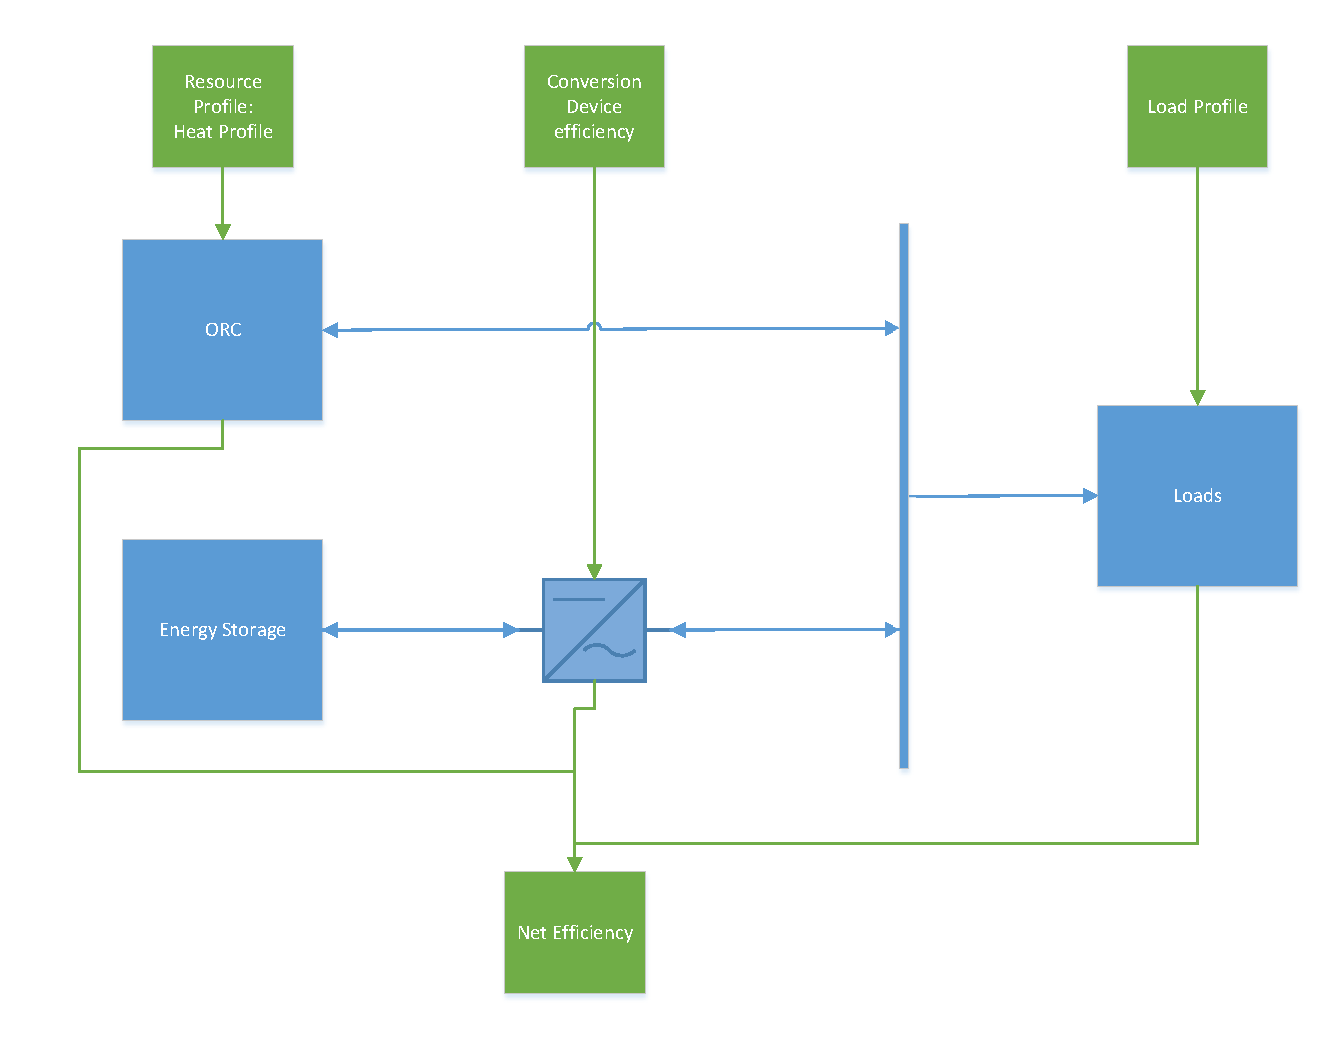
\includegraphics[width=\textwidth]{figures/Abridged Pilgrim Model Flow diagram - AC bus.pdf} 
	%\includegraphics[width=\textwidth]{figures/SimpleFlowDiagram.pdf}

\end{figure}

\section{Organic Rankine Cycle Generator}
The ORC generator block links the thermal, mechanical, and electric components of them model. The thermal properties of the fluids were obtained from the CoolProp library. \cite{Bell2014}
\subsection{Evaporator and Condenser}
The evaporator and the condenser are both represented using a heat exchanger script.  The function takes as inputs parameters about the high and low temperature fluids, specifically the inlet temperatures ($\si{\kelvin}$), mass flow rates ($\si{\kilogram\per\second} $), inlet pressures ($\si{\pascal}$), and fluid names, as well as parameters about the exchanger itself such as the overall heat transfer coefficient ($\si{\watt\per\kelvin\per\meter\squared}$), the heat transfer area ($\si{\meter\squared}$), and the heat exchanger type (e.g. counter or parallel flow). The function output is made up of the heat flow rate ($\si{\watt}$), and the temperatures at the outlets ($\si{\kelvin}$).

In order to calculate the desired values, the Number of Transfer Units (NTU) method is used. Described in The Fundamentals of Heat and Mass Transfer, \cite{Incropera} this process calculates the output heat flow, $Q$, relative to a theoretical maximum heat flow, $Q_{max}$. This potential heat flow would be realized using an infinitely long counter flow geometry and is calculated as 
\begin{equation}
Q_{max} = C_{min}\left(T_{h,i} - T_{c,i}\right)
\end{equation}
where $C_{min}$ is the smaller heat capacity rate of the hot and cool fluids and $T_{h,i}$ and $T_{c,i}$ are the inlet temperatures of hot and cool fluids respectively. The two heat flows are related by the effectiveness, $\epsilon$, which is defined as $\epsilon \equiv \frac{Q}{Q_{max}}$. The value of $\epsilon$ is a function of the ratio of the fluids' heat capacities, $C_r = \frac{C_{min}}{C_{max}}$, as well as the exchanger's Number of Transfer Units, $NTU = \frac{U*A}{C_{min}}$, where $U$ is the overall heat transfer coefficient and $A$ is the total heat transfer area. Additionally, the direction of fluid flow changes the method of calculation. In parallel flow heat exchangers, the effectiveness is calculated as
\begin{equation}
\epsilon = \frac{1 - \exp\left[-NTU\left(1 + C_r\right)\right]}{1 + C_r}
\end{equation}
while counter flow devices use
\begin{equation}
\epsilon = \frac{1 - \exp\left[-NTU\left(1 - C_r\right)\right]}{1 - C_r\exp\left[-NTU\left(1 - C_r\right)\right]}
\end{equation}
to calculate the value.

Within this script there are certain assumptions made in order to calculate the output values. Ambient temperature and associated heat flow to the external environment is not accounted for.

\subsubsection{Expander and Pump}

\subsection{Induction Generator}

\section{Load}

\section{Inverter and Storage}